\documentclass[12pt]{article}
\usepackage{fullpage}
\usepackage{lscape}
\usepackage[top=2cm, bottom=4.5cm, left=2.5cm, right=2.5cm]{geometry}
\usepackage{amsmath,amsthm,amsfonts,amssymb,amscd}
\usepackage{lastpage}
\usepackage{enumerate}
\usepackage{fancyhdr}
\usepackage{mathrsfs}
\usepackage{graphicx}
\usepackage{subcaption}
\usepackage{listings}
\usepackage{hyperref}
\usepackage{titlesec}
\usepackage[T1]{fontenc}
\usepackage[utf8]{inputenc}
\usepackage{palatino}
\usepackage{booktabs}
\usepackage[dvipsnames]{xcolor}
\usepackage{enumitem}

\definecolor{grey}{gray}{0.6}
\lstset{
    escapeinside={(*@}{@*)},
}

\newcommand{\SubItem}[1]{
    {\setlength\itemindent{15pt} \item[-] #1}
}

\newcommand\twoitems[2]{%
\item#1%
\hspace{20pt}%
\labelitemi
\hspace{\labelsep}#2
}

\setcounter{secnumdepth}{4}
\titleformat{\paragraph}
{\normalfont\normalsize\bfseries}{\theparagraph}{1em}{}
\titlespacing*{\paragraph}
{0pt}{3.25ex plus 1ex minus .2ex}{1.5ex plus .2ex}

\hypersetup{%
  colorlinks=true,
  linkcolor=blue,
  linkbordercolor={0 0 1}
}

\lstdefinestyle{C++}{
    language        = C,
    frame           = lines, 
    basicstyle      = \footnotesize\ttfamily,
    keywordstyle    = \color{blue},
    stringstyle     = \color{olive},
    commentstyle    = \color{red}\ttfamily,
    breaklines      = true,
    tabsize         = 2
}

\setlength{\parindent}{0.0in}
\setlength{\parskip}{0.05in}

\newcommand\code{\texttt}
\newcommand\course{COMP0019}
\newcommand\hwnumber{}                   
\pagestyle{fancyplain}
\headheight 35pt
\lhead{\NetIDa}
\lhead{\course}                 
\chead{\textbf{\Large Assessment \hwnumber}}
\rhead{\today}
\lfoot{}
\cfoot{}
\rfoot{\small\thepage}
\headsep 1.5em

\graphicspath{{./imgs/}}

\renewcommand{\thesubsection}{\thesection.\alph{subsection}}
\renewcommand{\thesubsubsection}{\thesubsection.\roman{subsubsection}}


\begin{document}

\section{}

\subsection{}

\subsubsection{}
\label{section:1ai}

Consider Core i19's support for the virtual memory with a page size of 4096 bytes. This would consume the $\log_2(4096) = 12$ least significant bits of the virtual address. 

Hence,
$$\mathtt{VPO = PPO} = 12\; \mathtt{bit}$$

Consider the proposed L1 cache by the colleague, 8-way associative cache with 64 byte blocks, 256 KB in total. Thus, the cache would have
$$ \frac{256\; \mathtt{KB}}{64\; \mathtt{B/block} \times 8 \; \mathtt{block/line}} = 512\; \mathtt{line}$$
Consuming Cache Index bits of,
$$ \mathtt{CI} = \log_2(512) = 9\; \mathtt{bit} $$
Consuming Cache Offset bits of,
$$ \mathtt{CO} = \log_2(64) = 6\; \mathtt{bit} $$

We compare the bit width as $\mathtt{CI + CO} = 9+6=15 > \mathtt{PPO} = 12 $. As shown in Figure \ref{fig:1a} below, this violates the restriction of VIPT (Virtually Indexed Physically Tagged) cache, as the Cache Set Index $CI$ would span across Page Number (3 bits) and Page Offset (6 bits).

\begin{figure}[h!]
  \makebox[\textwidth][c]{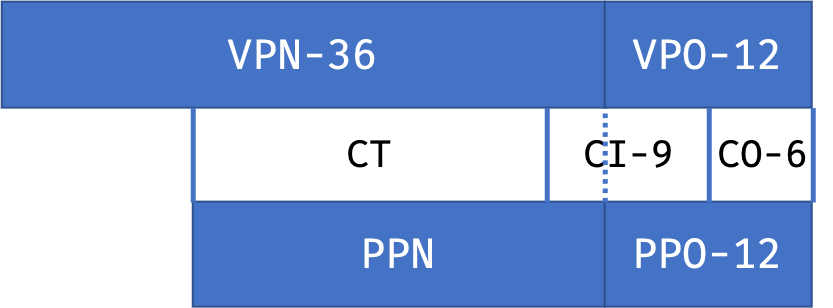
\includegraphics[width=0.5\textwidth]{imgs/1a.png}}
  \caption{Demonstration of bits layout in the Core i19 system}
  \label{fig:1a}
\end{figure}

It is important to recognise that the TLB translation of VPN \textrightarrow{} PPN happens \textbf{at the same time} as the L1 cache figures out which set this line belongs with CI. After the TLB translation, the L1 Cache would have already targeted the Cache set to look into and compare the tag with each cache line thereafter.

In the case of having two processes mapping the same virtual address to two different physical addresses, it would result in a potential problem named cache homonym. 

\paragraph*{Cache Homonym Example}

Consider two processes that map virtual address VPN:VPO to PPN1:PPO and PPN2:PPO, respectively; the L1 Cache would take \textbf{the last 3 bits of VPN and the first 6 bits of VPO} for the set lookup, which would be identical for both processes.

Now that the TLB translates VPN \textrightarrow{} PPN, we are looking at the same Cache set in the L1 Cache. Consider a case where the physical address only differs in \textbf {the last 3 bits of PPN1 and PPN2}; we would notice that the Cache Tag is also identical! This creates a problem here as we are looking at two different physical address that maps to the same cache line. The issue lies in the fact that the cache tag itself here would be insufficient to identify the address uniquely.

\subsubsection{}

The Linux kernel is a preemptive multitasking kernel (contrary to uni-kernel). Since each process has its own mapping in its page table, it is very possible that they could map the same virtual address to different physical pages. 

For example, in the text section, two different processes would map the same virtual address ($\mathtt{0x400000}$) to their own code, respectively, which would very likely be in different physical addresses. 

Another example would be an address in the middle of the virtual memory space that belongs to the heap of each process (note that it is not the same heap, just the same virtual address). Each process can arbitrarily map the allocated heap virtual address to anything it needs during the execution process. So, again, it is very likely to map the same virtual address to different physical addresses.

\subsection{}

\subsubsection{}

With reference to the analysis in section \ref{section:1ai}, we illustrate the issue cache synonym that happens when two processes map the same physical address to two different virtual addresses.

\paragraph*{Cache Synonym Example}

Consider two processes that map VPN1:VPO and VPN2:VPO both to PPN:PPO. Note that the VPO must match with PPO, due to the address translation process only happens at the top bits of the address. When the L1 Cache is determining which set to look for, again, it takes \textbf{the last 3 bits of VPN1/VPN2 and the first 6 bits of VPO}. Consider a case where the VPN1 differs from VPN2 in the last three digits; the L1 Cache would be looking at two completely different sets given the different Cache Set Index.

After the address translation, we would have the same PPN; the L1 Cache would have the same tag but in different sets. We observe that the same physical address is now mapped to the same tag but different sets in the L1 Cache! Same data getting cached in several different sets (and different lines due to set difference) would yield unexpected results. Consider a write-back cache where the two copies are modified simultaneously; both processes would not see each other's modifications due to different sets/lines. Moreover, the Cache would not be able to determine what to write when finally writing the two (or more) cache lines that belong to the same physical address to the lower level.

\subsubsection{}

Even for a single process, we can also map the same physical address to multiple virtual addresses. It would also be possible for multiple processes.

For example, \texttt{glibc}'s code, as used by multiple processes, can retain one copy in the physical memory while being mapped to different virtual addresses of various processes as needed. This is the standard behaviour of the Linux kernel to save memory resources.


\subsection{}

To avoid the aforementioned issues, we need to design a VIPT cache. The key to do so is to make sure the untranslated bits (VPO/PPO) of the address fits in both Cache Set Index and Cache Block Offset. 

Let $s$ be the bit width of set ($S = 2^s$ sets), $e$ be the bit width of lines per set ($E = 2^e$ lines), and $b$ be the bit width of bytes per line ($B = 2^b$ bytes).

Given the virtual page size of $P$ bytes, let $2^p = P$, the VPO shall be $p$-bit wide. Thus $s + b \leq p$. The cache capacity shall be $S \times E \times B$, where $S \times B \leq P$.

Now the greatest L1 data cache capacity is dependent on the associativity of the Cache. Thus, we conclude, on a $E$-way set associative Cache, for it to be VIPT,
$$ C_{greatest} = P \times E$$

\newpage
\section{}

\subsection{}
First, her implementation would be erroneous when \texttt{strcmp()} encounters a 0, which could mean both the null terminator \texttt{'\textbackslash0'} and the data symbol $\mathtt{0b00}$. Thus, her comparison of two long strings would most likely terminate early when any of them has a $\mathtt{0b00}$ symbol in the middle.

Second, her implementation would go out of memory bounds when \texttt{strcat()} two strings together. As specified in the problem, she only allocates two bytes of memory for a new C string. When she concatenates the two strings together, \texttt{strcat()} will not check for memory boundary, nor would it allocate new memory at the end of the destination string. Most likely, when she accumulated a long enough string, it would write to an invalid page and returns a segfault.

\subsection{}

\subsubsection{}

For implementation 1, it consumes 1 byte for each symbol. It also needs one more byte for the $\mathtt{0xff}$ terminator. Hence, the string itself consumes $n + 1$ bytes. However, to be comparable, we would need a pointer that points to the \texttt{malloc}'d string buffer, which would be 8 bytes on an x86-64 system. In total, this implementation consumes $n + 1 + 8 = n + 9$ bytes.

For implementation 2, it consumes 8 bytes for \texttt{char *s;}, and 2 bytes for \texttt{unsigned short len;}, but another 6 bytes for the 8-byte alignment requirement. Thus, the \texttt{struct symstring} would consume $8 + 2 + 6 = 16$ bytes. The n symbol string would not need a terminator anymore, as the length is encoded in the struct. In total, that would be $n + 16$ bytes.

Implementation 1 is more memory efficient. Compared to implementation 2, where it uses the extra memory overhead \texttt{struct} to store the string length (with additional alignment), implementation 1 only needs one more \texttt{char 0xff} to act as the terminator.

\subsubsection{}

Implementation 2 is more CPU-efficient when appending the newly read input symbol to the end. 

For implementation 1, since we only have the pointer to the start of the section provided by \texttt{malloc}, we would need $O(n)$ (n being the string length) time to traverse the string and find the terminator. Then, we can make changes to the terminator and append strings thereafter.

For implementation 2, we already have the length in the \texttt{struct}. We can essentially "fly" to end and append at \texttt{char* nextsym = s + len}. This is a constant time operation with $O(1)$ time. Thus, it shall be more CPU-efficient.

Note that when appending new symbols, we shall be wary of the total allocated memory size and make sure to \texttt{realloc} when necessary.

\subsubsection{}

In implementation 1, we \texttt{malloc} string blocks in the table as we go along encoding the file. Since the LZW encoder never deallocate an individual symbol once it has been added, we can instead \texttt{malloc} a reasonably large block of memory at the beginning. As we go along and grow the table, we can \texttt{realloc} the block if needed.

This alternative approach saves both memory and CPU time. Memory wise, we have a lower dynamic allocation overhead. CPU wise, besides keeping each \texttt{malloc} calls, we can quickly iterate over the table, as the data in the same block exhibits better spatial locality. Moreover, \texttt{realloc} would try to expand the block if possible. Only if the block is not expandable would it find another larger block and move our memory there. 

\subsection{}

This second bullet point is incorrect. She should \textbf{increment the \texttt{currwidth} on adding a longer-bit entry to the table}. It can be too late to increment \texttt{currwidth} when the encoder needs to output longer bits of code.

\paragraph*{Error Example}

Let the symbols be 0, 1, 2, 3.

We construct a symbol string: \texttt{0 1 2 3 0 2 1 3}

At the beginning, we should have
\begin{itemize}[topsep=0pt]\itemsep-0.6em 
    \item 0 \textrightarrow{}000
    \item 1 \textrightarrow{}001
    \item 2 \textrightarrow{}010
    \item 3 \textrightarrow{}011
\end{itemize}

We use "|" to show the encoder/decoder progress below.

\textbf{Encoder Stage:} \texttt{0 | 1 2 3 0 2 1 3}
\newline Output: \texttt{000}
\newline New Table Entry: N/A

\textbf{Encoder Stage:} \texttt{0 1 | 2 3 0 2 1 3}
\newline Output: \texttt{000 001}
\newline New Table Entry: 0 1 \textrightarrow{} 100

\textbf{Encoder Stage:} \texttt{0 1 2 | 3 0 2 1 3}
\newline Output: \texttt{000 001 010}
\newline New Table Entry: 1 2 \textrightarrow{} 101

\textbf{Encoder Stage:} \texttt{0 1 2 3 | 0 2 1 3}
\newline Output: \texttt{000 001 010 011}
\newline New Table Entry: 2 3 \textrightarrow{} 110

\textbf{Encoder Stage:} \texttt{0 1 2 3 0 | 2 1 3}
\newline Output: \texttt{000 001 010 011 000}
\newline New Table Entry: 3 0 \textrightarrow{} 111

\textbf{Encoder Stage:} \texttt{0 1 2 3 0 2 | 1 3}
\newline Output: \texttt{000 001 010 011 000 {\color{blue}0010} }
\newline Wrong: \ \texttt{000 001 010 011 000 {\color{red}010} } (no input longer than 3 bits detected)
\newline New Table Entry: 0 2 \textrightarrow{1000}

\textbf{Encoder Stage:} \texttt{0 1 2 3 0 2 1 | 3}
\newline Output: \texttt{000 001 010 011 000 0010 {\color{blue}0001} }
\newline Wrong: \ \texttt{000 001 010 011 000 010 {\ \color{red}001} } (similar as above)
\newline New Table Entry: 2 1 \textrightarrow{1001}

\textbf{Encoder Stage:} \texttt{0 1 2 3 0 2 1 3 |}
\newline Output: \texttt{000 001 010 011 000 0010 0001 {\color{blue}0011} }
\newline Wrong: \ \texttt{000 001 010 011 000 010 001  {\ \ \color{red}011} } (similar as above)
\newline New Table Entry: 1 3 \textrightarrow{1010}

With the error-nous encoder, we now have the compressed string :

\texttt{\color{red}000 001 010 011 000 010 001 011}

The correct compressed string shall be:

\texttt{\color{blue}000 001 010 011 000 0010 0001 0011}

We initialise the table entry as below and start decoding
\begin{itemize}[topsep=0pt]\itemsep-0.6em 
    \item 0 \textrightarrow{}000
    \item 1 \textrightarrow{}001
    \item 2 \textrightarrow{}010
    \item 3 \textrightarrow{}011
\end{itemize}

\textbf{Decoder Stage:} \texttt{000 | 001 010 011 000 010 001 011}
\newline Output: \texttt{0}
\newline New Table Entry: N/A

\textbf{Decoder Stage:} \texttt{000 001 | 010 011 000 010 001 011}
\newline Output: \texttt{0 1}
\newline New Table Entry: 0 1 \textrightarrow{} 100

\textbf{Decoder Stage:} \texttt{000 001 010 | 011 000 010 001 011}
\newline Output: \texttt{0 1 2}
\newline New Table Entry: 1 2 \textrightarrow{} 101

\textbf{Decoder Stage:} \texttt{000 001 010 011 | 000 010 001 011}
\newline Output: \texttt{0 1 2 3}
\newline New Table Entry: 2 3 \textrightarrow{} 110

\textbf{Decoder Stage:} \texttt{000 001 010 011 000 | 010 001 011}
\newline Output: \texttt{0 1 2 3 0}
\newline New Table Entry: 3 0 \textrightarrow{} 111

{\color{red} last entry in 3 bits, time to increment bit width and expect 4-bit symbols now}

\textbf{Decoder Stage:} \texttt{000 001 010 011 000 {\color{red}(010 0)} | 01 011}
\newline Output: \texttt{0 1 2 3 0 {\color{red}0 1}}
\newline New Table Entry: 0 0 \textrightarrow{} 1000

\textbf{Decoder Stage:} \texttt{000 001 010 011 000 (010 0) {\color{red}(01 01)} | 1}
\newline Output: \texttt{0 1 2 3 0 0 1 {\color{red}1 2}}
\newline New Table Entry: 0 1 1 \textrightarrow{} 1001

\textbf{Decoder Stage:} \texttt{000 001 010 011 000 (010 0) (01 01) {\color{red}1}}
\newline Output: \texttt{0 1 2 3 0 0 1 1 2}
\newline \texttt{Invalid decoder input: aborting}, why is there only 1 bit left?

Hence, the decoder outputs an error, with the output string \texttt{0 1 2 3 0 0 1 1 2} different from \texttt{0 1 2 3 0 2 1 3}.

In conclusion, we showed that the encoder should have increased the \texttt{currwidth} on adding the first longer-bit table entry.


\newpage
\section{}

\subsection{}

\begin{lstlisting}[style=C++, label={lst:3a}, caption={Weensy OS defined constants},captionpos=b]
// kernel.h
// First application-accessible address
#define PROC_START_ADDR         0x100000
// Virtual memory size
#define MEMSIZE_VIRTUAL         0x300000

// x86-64.h
#define PAGEOFFBITS     12                   // # bits in page offset
#define PAGESIZE        (1 << PAGEOFFBITS)   // Size of page in bytes
#define PAGEINDEXBITS   9                    // # bits in a page index level
#define NPAGETABLEENTRIES (1 << PAGEINDEXBITS) // # entries in page table page
typedef uint64_t x86_64_pageentry_t;
typedef struct __attribute__((aligned(PAGESIZE))) x86_64_pagetable {
    x86_64_pageentry_t entry[NPAGETABLEENTRIES];
} x86_64_pagetable;
\end{lstlisting}

The Weensy OS has the following constants shown in Listing \ref{lst:3a}. At the lowest level, a level 4 page table maps to 
$$2^{12} \times 2^{9} = 2^{21} = \mathtt{0x200000} \; \text{addresses}$$
Thus, the level 4 page tables covers the address range 
$$[\mathtt{0x000000},\mathtt{0x200000 - 1}], [\mathtt{0x200000},\mathtt{0x400000 - 1}], ...$$
To cover \texttt{PROC\_START\_ADDR}($\mathtt{0x100000}$) to \texttt{MEMSIZE\_VIRTUAL - 1}($\mathtt{0x300000 - 1}$), we need 2 level 4 page tables, covering $[\mathtt{0x100000},\mathtt{0x200000 - 1}]$ and $[\mathtt{0x200000},\mathtt{0x300000 - 1}]$ respectively. These 2 level 4 page tables are pointed to by the first two PTEs in a level 3 page table. The level 3 page table is pointed to by the first PTE of a level 2 page table, and similarly for the level 2 and a level 1 page table.

There are a total of $2 + 1 + 1 + 1 = 5$ page tables. 

For each existing page table, we allocated $2^9$ PTEs, regardless of each PTE is used or not. That would amount to a total of $5 \times 2^9$ PTEs.

Each PTE is a \texttt{uint64\_t}, thus consuming $8$ bytes of memory. The total amount of memory consumed is $5\times 2^9 \times 8 = 5 \times 2^{12}$ bytes.

Each page is of \texttt{PAGE\_SIZE}, which is $2^{12}$ bytes. Hence, we can conclude that in total page tables at level 1, 2, 3, 4 takes up 5 pages of memory.


\subsection{}

\texttt{kernel\_pagetable = \&kernel\_pagetables[0];} This line sets the global kernel page table pointer to the address of the level 1 page table.

\texttt{memset(kernel\_pagetables, 0, sizeof(kernel\_pagetables));} The \texttt{memset()} call wipes the kernel page tables of all 4 levels and reset them to 0.

\texttt{kernel\_pagetables[0].entry[0] = ...;} This line points the first entry of the level 1 page table to the level 2 page table. Also, it sets the \texttt{Present}, \texttt{Writable} and \texttt{User Accessible} permission bits to 1 for the first entry of the level 1 page table.

\texttt{kernel\_pagetables[1].entry[0] = ...;} This line does the similar set of operations as the line above. The first entry of the level 2 page table now points to the level 3 page table. It is also configured with the same set of permission bits.

\texttt{kernel\_pagetables[2].entry[0] = ...;} Similarly, this operation connects the first entry of the level 3 page table with the first level 4 page table, with the same set of permission bits.

\texttt{kernel\_pagetables[2].entry[1] = ...;} This operation now connects the second entry of the level 3 page table with the second level 4 page table, with the same set of permission bits.

\texttt{virtual\_memory\_map(...);} After properly connecting the virtual memory page tables, we then call the \texttt{virtual\_memory\_map()} utility function to map the virtual addresses in range $[\mathtt{0x000000},\mathtt{0x200000 - 1}]$ to its identical physical addresses (which is the entire physical address space).

\texttt{lcr3((uintptr\_t) kernel\_pagetable);} Lastly, we store the address of the level 1 page table in the \texttt{\$cr3} register. 



\newpage
\section{}

\subsection{}

\subsubsection{}

As described above, we consider \texttt{malloc()/free()} a function that does the following:
\begin{itemize}[topsep=0pt]\itemsep-0.6em 
    \item \texttt{spinlock.lock();}
    \item \texttt{// operates on the heap}
    \item \texttt{spinlock.unlock();}
\end{itemize}

Consider the parent process's two threads, $T_1$ is in the middle of a \texttt{malloc()}, while $T_2$ is \texttt{fork()}-ing a child process. Note that the lock is now in the hands of $T_1$'s \texttt{malloc()}. 

As described above, calling \texttt{fork()} on a multi-threaded program would \textbf{only fork the single thread that actually called it}. However, \textbf{the entire virtual address space of the parent process is replicated in the child}, including the states of spinlocks. In other words, only $T_{2forked}$ exists, while $T_{1forked}$ is not there anymore to unlock its locked $\mathtt{spinlock}_{forked}$. Thus, when $T_{2forked}$ invokes \texttt{malloc()} later on in the logic flow, the locked $\mathtt{spinlock}_{forked}$ (but never can be unlocked) would result in a deadlock and hangs the child process.

\subsubsection{}

No, she is not correct.

Being async-signal-safe a function means that the function is either reentrant or uninterruptible by signals (uninterruptible system calls). If a function is reentrant, it can be interrupted in the middle of execution and safely called again before completing its previous invocation. \texttt{malloc()} would clearly not be able to achieve this as it operates on a globally shared data structure.

Consider a single-threaded process where \texttt{malloc()} is invoked normally, and in its signal handlers. Signals can arrive at any time of execution, hence asynchronous. In the case where a signal arrives during the \texttt{malloc()} process in the logic flow, the signal handler would be invoked. 

If it is a thread-safe \texttt{malloc()}, the logic flow \texttt{malloc()} would be holding the heap lock, waiting for the signal handler to finish. The signal handler, on the other hand, is waiting for its \texttt{malloc()} to acquire the heap lock. This results in an unfortunate deadlock situation.

Now we consider removing the locks of the \texttt{malloc()} (or if we use a reentrant lock in C++). Then, the signal handler's \texttt{malloc()} (in the same thread as the logic flow) would encounter a half-modified heap state, and could potentially corrupt the heap structure by allocating new blocks on top of it.

In all, as we have shown, \texttt{malloc()} is \textbf{not async-signal-safe}, with or without the process-wide spinlock on the heap.

\subsection{}

\subsubsection{}

The string \texttt{"Hello"} is printed twice due to the output is line-buffered in C's Standard I/O.

When the first \texttt{printf("Hello")} is called, the string \texttt{"Hello"} is put into the buffer for \texttt{stdout}. Since the \texttt{stdout} is line-buffered by default, we would not see the string on the screen yet.

Then the \texttt{fork()} happens. As mentioned previously, \texttt{fork()} copies the entire virtual address space to the child in a copy-on-write fashion, including the \texttt{stdout} buffer. Now, we have two copies of the \texttt{stdout} buffer, both with the string \texttt{"Hello"}.

The child process than calls \texttt{printf("Child goodbye\textbackslash n")} with a newline. Since there is a new line, the whole string in the child's buffer \texttt{"HelloChild goodbye"} would be presented on the console. The same happens for the parent process as well (\texttt{"HelloParent goodbye"}). Therefore, there are two \texttt{"Hello"}s in total.

\subsubsection{}

Here we offer two ways to force the output \texttt{"Hello"} to be generated once.

First, we can simply turn off the buffer on the \texttt{stdout} stream as shown in the code listing \ref{lst:4bii-nobufstdio}. Thus everything printed using Standard I/O to \texttt{stdout} will be turned into a \texttt{write()} system call immediately. 

\begin{lstlisting}[style=C++, label={lst:4bii-nobufstdio}, caption={Turn off buffer for \texttt{stdout}},captionpos=b]
#include <stdio.h>
#include <unistd.h>

int main () {
  (*@\textbf{setvbuf(stdout, NULL, \_IONBF, 0);}@*)
  printf("Hello");
  if (fork() == 0) {
    printf("Child goodbye\n");
  } else {
    printf("Parent goodbye\n");
  }
  return 0;
}
\end{lstlisting}

The other way would be to flush the \texttt{stdout} buffer before \texttt{fork()}, as shown in listing \ref{lst:4bii-flush}.

\begin{lstlisting}[style=C++, label={lst:4bii-flush}, caption={Flush the \texttt{stdout} buffer before \texttt{fork}},captionpos=b]
#include <stdio.h>
#include <unistd.h>

int main () {
  printf("Hello");
  (*@\textbf{fflush(stdout);}@*)
  if (fork() == 0) {
    printf("Child goodbye\n");
  } else {
    printf("Parent goodbye\n");
  }
  return 0;
}
\end{lstlisting}


\newpage
\section{}

\subsection{Web Browser}
To build a web browser, we favour processes over threads.

Analysing the task requirement, a browser needs to run multiple browsing tabs at the same time. Each browsing tab would have its own set of network communications and webpage rendering tasks. In modern-day browsers, each tab also needs a safe environment for JavaScript execution. Also, the browser could have multiple UIs if there are multiple windows opened. 

Therefore, we design a multi-process system for the web browser. Each tab is a single process that provides an HTML/CSS rendering environment with its own isolated JavaScript sandbox. On top of that, we design several controller/servicing processes that offer essential service to the tab processes. These include a main controller process that handles network I/O, file I/O, browser UIs and inter-process communications, a plugin process that handles browser plugins, and many other utility processes as needed (e.g. a GPU process). We plan to enable the Inter-Process Communication (IPC) via several non-blocking FIFO special files (named pipes). This is to ensure that each communication channel has a name and can be referred to and organised efficiently across processes.

The main advantage of this multi-process design is to maintain isolation across tabs. Since processes do not share memory by default, any malicious JavaScript code within one tab process would not be able to fetch any information directly from other websites users are using (e.g. \url{paypal.com}). Also, using processes to isolate tabs brings more stability to the browser. Consider the case where poorly-written JavaScript crashes one of the tab processes, other tabs would remain intact, and the general operation of the browser would remain unaffected. 

Note that in our design, all tabs' I/Os are handled by the same main process. This design intends to create a privilege difference between processes handling any hostile external webpage code and the core process handling system resources. Since each process has its own permission, we can disable file and network I/O as a whole on tab processes to ensure security.

On the other hand, implementing the browser with a multi-process design could be slower. On clicking a new tab, for example, the system would have to do more \texttt{clone()} work from the original process (e.g. clone a separate copy of memory space) than a thread-based design. Also, 
creating IPC FIFOs across tabs processes, and the main process would make several system calls (\texttt{mkfifo()}), which would be slower than threads reading off a shared heap space.

\subsection{Web Server}
We prefer a multi-threaded design over a multi-process design on a typical web server.

As per the requirements, the webserver serves multiple requests from clients concurrently. The server programs generally run in a more trusted environment than the browser, as the code in execution would be written by a trusted developer. Hence, there is not as much isolation/sandbox necessity as the browser would need. However, the server could potentially face a high number of concurrent client requests, and should be able to handle as many clients as possible.

With that in mind, we design a multi-threaded structure for a web server. The (single) process executes with the main thread and a thread pool. A new client request would be put into a blocking queue, waiting to be serviced by an available thread in the pool. The main thread monitors the thread statuses, launches threads in the pool, and manages the IPC communications with databases. The shared memory across threads shall marked \texttt{atomic}, or relevant code sections shall be locked by a \texttt{mutex} or \texttt{spinlock}.

The main advantage of this design would be service performance. Since it is very common for each thread to share certain service data (e.g. stocks left in the warehouse), the memory sharing across threads would significantly reduce the fetching overhead. As threads themselves consumes fewer system resources, we can potentially spawn more threads than processes when saturating the system workload.

Note that we use a thread pool instead of spawning/destroying thread per request. This is favourable as it eliminates the overhead of \texttt{pthread\_create()} and \texttt{pthread\_join()} during each service period. 

However, there are several downsides to using this multi-threaded model. If the code is poorly written and causes a segment fault in one thread, the whole process would be terminated. This would not happen in a multi-process server, as only one of the worker processes will be terminated. Another disadvantage of using threads lies in difficulty to limit system resources per thread. Consider a case where the request is time-consuming (possibly an attack), and one of the threads is taking much longer than expected or runs into an infinite loop; the thread cannot be easily timed and terminated. The master process/kernel could simply enforce an operation timeout on that particular request if it were a process.

\subsection{Key-Value Pair Storage Server}

As for the key-value pair storage server, we favour a multi-threaded model over a multi-process model.

Regarding the design requirements, the storage servers need to provide data read and write service for multiple clients. The requirement explicitly mentions the database Redis; hence we assume performance is one of the primary concerns of this design. It is also crucial for a database to maintain data integrity and ensure no corruption happens during large amounts of concurrent operations.

We propose a multi-threaded design of such a database, with one single main operation thread, one queue management thread and several utility threads that does garbage collection. The main thread handles all read and write events to the database. All reads and writes requests to the storage server are queued by their time of arrival and dispatched to the main operation thread. To support expiry utility, we have utility threads that free expired key-value pairs. Note that the main operation thread shall disregard any information expired to avoid concurrent operation on the same data with the garbage collector.

The main advantage here is a guarantee of data integrity. With one single operation thread on all data, there shall be no race conditions or visibility issues. Every modification is visible to all queries thereafter chronologically, and there would never be simultaneous updates to the same data. 

Another key advantage of this design is the performance. In the case of an in-memory database like Redis, the memory I/O is much faster than disk I/O, implying that a typical read/write operation shall take a minimal amount of CPU cycles. Thus, the main operation thread would not be blocked for a prolonged period. When the server reaches maximum operation capacity, it is far more likely to be memory-I/O-bounded or network-I/O-bounded rather than CPU-bounded. Thus, we argue that one single main operation thread would be enough.

As implied previously, the major downside of such a design happens when the server encounters a long-running command that blocks the operation thread for a long time. Simply put, there would be no other way to access any database information, not even reading, as the command blocks the only thread. We can use a separate read thread to mitigate this situation. However, with this approach, there will no longer be any guarantee of whether the value read is up-to-date.

\subsection{Process VS Thread in Linux}

As an end note, it is worth mentioning that Linux uses a 1-1 threading model. From the kernel's perspective, there is no distinction between a thread or a process. They are simply "runnable tasks" and uses the same \texttt{struct task\_struct}. Thus, as implied previously, \texttt{fork()} and \texttt{pthread\_create()} would create "tasks" with the same system call \texttt{clone()}. The difference between a process and a thread lies in the \texttt{cl\_args} set during the system call. Technically speaking, we can create half-process, half-thread in Linux by tuning the clone flags.

Although \texttt{fork()} requires more processing than \texttt{pthread\_create()} in its extra copying of data structures (e.g. Copy-on-Write mappings of memory), these costs are minimal comparable with the program's execution. Also, switching between "runnable tasks" are largely similar in the kernel, with only a tiny bit of performance edge for threads. 

\end{document}